\Aufgabe[e]{~} {
%Plot each of the following functions in a coordinate system individually,
%label the data axes and highlight significant values.
Stellen Sie jede der folgenden Funktionen einzeln in einem Koordinatensystem dar, beschriften Sie die Datenachsen und heben Sie signifikante Werte hervor (z.B. Maxima/Minima, Nullstellen, usw.).

\begin{abc}
\item $p_1(x)=2x-1$

\item $p_2(x)=(x-2)^2-1$

\item $p_3(x)=x^3$

\item $p_4(x)=-x^3$


\item $f_1(x)=\sin(x+\frac{\pi}{2})$

\item $f_2(x)=-\cos(x)$

\item $f_3(x)=\sin(x)$

\item $f_4(x)=\tan x$


\item $g_1(x)=\sqrt{x}$

\item $g_2(x)=\displaystyle \frac{1}{x}$

\item $g_3(x)=\displaystyle \frac{1}{x^2}$


\item $h_1(x)=\ln x$

\item $h_2(x)=\ln x +1$

\item $h_3(x)=\ln(x+1)$


\item $i_1(x) = \exp(x)$

\item $i_2(x) = \exp(-x)$

\end{abc}

}


\Loesung{

\textbf{a)} $p_1(x)=2x-1$

\begin{minipage}{\linewidth}
\centering

\begin{tikzpicture}
\begin{axis}[
axis lines=middle,
clip=false,
xmin=-pi,
xmax=3*pi,
ymin=-5.9,
ymax=5.9,
xlabel=$x$,
ylabel=$f(x)$,
xticklabel style={black}
]

\addplot[domain=-1.7:2.9,samples=200,blue]{2*x-1}
node[right,pos=.9,font=\footnotesize]{$p_1(x)$};

\end{axis}
\end{tikzpicture}

\end{minipage}


\bigskip
\textbf{b)} $p_2(x)=(x-2)^2-1$

\begin{minipage}{\linewidth}
\centering

\begin{tikzpicture}
\begin{axis}[
axis lines=middle,
clip=false,
xmin=-pi,
xmax=3*pi,
ymin=-5.9,
ymax=5.9,
xlabel=$x$,
%ylabel=$y$,
xticklabel style={black}
]

\addplot[domain=-0.5:4.5,samples=200,blue]{(x-2)^2-1}
node[right,pos=.9,font=\footnotesize]{$p_2(x)$};

\end{axis}
\end{tikzpicture}

\end{minipage}

\newpage
\bigskip
\textbf{c)}  $p_3(x)=x^3$

\bigskip
\textbf{d)}  $p_4(x)=-x^3$


\begin{minipage}{\linewidth}
\centering

\begin{tikzpicture}
\begin{axis}[
axis lines=middle,
clip=false,
xmin=-pi,
xmax=3*pi,
ymin=-5.9,
ymax=5.9,
xlabel=$x$,
%ylabel=$y$,
xticklabel style={black}
]
\addplot[domain=-1.75:1.75,samples=200,blue]{x^3}
node[right,pos=.9,font=\footnotesize]{$x^3$};

\addplot[domain=-1.75:1.75,samples=200,red,densely dashed]{-x^3}
node[right,pos=.9,font=\footnotesize]{$-x^3$};

\end{axis}
\end{tikzpicture}

\end{minipage}

%\bigskip
\textbf{e)} $f_1(x)=\sin(x+\frac{\pi}{2}) = \cos(x)$

\bigskip
\textbf{f)} $f_2(x)=-\cos(x)$

\begin{minipage}{\linewidth}
\centering

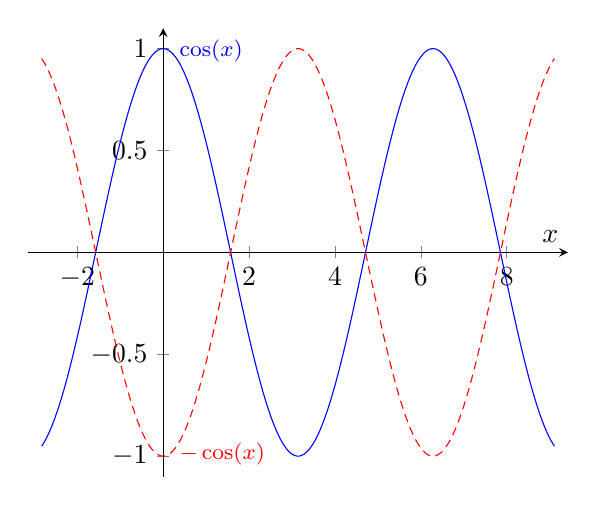
\begin{tikzpicture}
\begin{axis}[
axis lines=middle,
clip=false,
xmin=-pi,
xmax=3*pi,
ymin=-1.1,
ymax=1.1,
xlabel=$x$,
%ylabel=$y$,
xticklabel style={black}
]

\addplot[domain=-.9*pi:2.9*pi,samples=200,blue]{cos(deg(x))}
node[right,pos=.25,font=\footnotesize]{$\cos(x)$};

\addplot[domain=-.9*pi:2.9*pi,samples=200,red,densely dashed]{-cos(deg(x))}
node[right,pos=.25,font=\footnotesize]{$-\cos(x)$};

\end{axis}
\end{tikzpicture}

\end{minipage}

\newpage
\bigskip
\textbf{g)} $f_3(x)=\sin(x)$

\begin{minipage}{\linewidth}
\centering

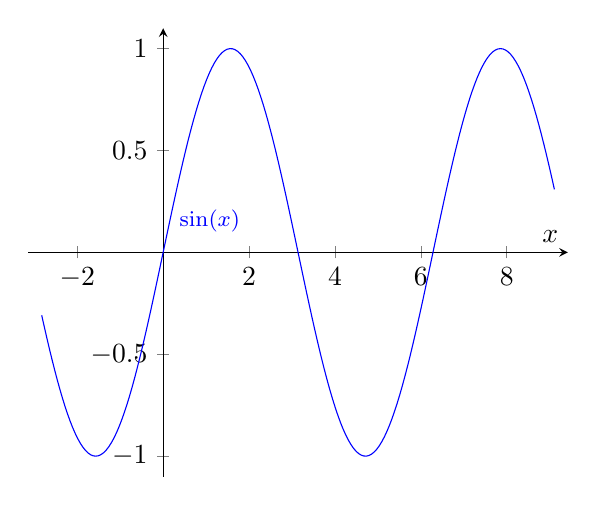
\begin{tikzpicture}
\begin{axis}[
axis lines=middle,
clip=false,
xmin=-pi,
xmax=3*pi,
ymin=-1.1,
ymax=1.1,
xlabel=$x$,
%ylabel=$y$,
xticklabel style={black}
]

\addplot[domain=-.9*pi:2.9*pi,samples=200,blue]{sin(deg(x))}
node[right,pos=.25,font=\footnotesize]{$\sin(x)$};


\end{axis}
\end{tikzpicture}

\end{minipage}

\bigskip
\textbf{h)} $f_4(x)= \tan x$

\begin{minipage}{\linewidth}
\centering

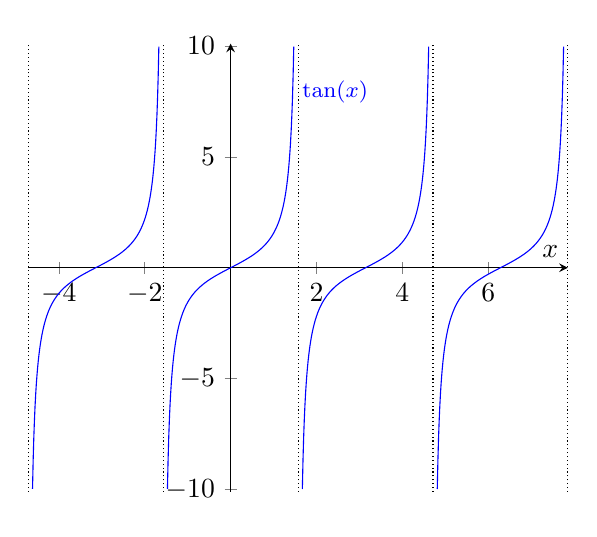
\begin{tikzpicture}
\begin{axis}[
axis lines=middle,
clip=false,
xmin=-1.5*pi,
xmax=2.5*pi,
ymin=-10.1,
ymax=10.1,
xlabel=$x$,
%ylabel=$y$,
xticklabel style={black}
]

\addplot[mark=none,black,densely dotted] coordinates {(-pi/2-pi, -10.1) (-pi/2-pi, 10.1)};

\addplot[domain=-pi/2+.1-pi:pi/2-.1-pi,samples=200,blue]{tan( deg(x) )};

\addplot[mark=none,black,densely dotted] coordinates {(-pi/2, -10.1) (-pi/2, 10.1)};

\addplot[domain=-pi/2+.1:pi/2-.1,samples=200,blue]{tan( deg(x) )}
node[right,pos=0.9,font=\footnotesize]{$\tan(x)$};

\addplot[mark=none,black,densely dotted] coordinates {(-pi/2+pi, -10.1) (-pi/2+pi, 10.1)};

\addplot[domain=-pi/2+.1+pi:pi/2-.1+pi,samples=200,blue]{tan( deg(x) )};

\addplot[mark=none,black,densely dotted] coordinates {(-pi/2+2*pi, -10.1) (-pi/2+2*pi, 10.1)};

\addplot[domain=-pi/2+.1+2*pi:pi/2-.1+2*pi,samples=200,blue]{tan( deg(x) )};

\addplot[mark=none,black,densely dotted] coordinates {(-pi/2+3*pi, -10.1) (-pi/2+3*pi, 10.1)};

\end{axis}
\end{tikzpicture}

\end{minipage}


\newpage
\bigskip
\textbf{i)} $g_1(x)=\sqrt{x}$

\begin{minipage}{\linewidth}
\centering

\begin{tikzpicture}
\begin{axis}[
axis lines=middle,
clip=false,
xmin=-1.1,
xmax=3.9,
ymin=-1.1,
ymax=3.9,
xlabel=$x$,
ylabel=$f(x)$,
xticklabel style={black}
]

\addplot[domain=0:3.7,samples=200,blue]{sqrt(x)}
node[right,pos=.1,font=\footnotesize]{$\sqrt{x}$};

\end{axis}
\end{tikzpicture}

\end{minipage}


\bigskip
\textbf{j)} $g_2(x)=\displaystyle \frac{1}{x}$

\bigskip
\textbf{k)} $g_3(x)=\displaystyle \frac{1}{x^2}$

\begin{minipage}{\linewidth}
\centering

\begin{tikzpicture}
\begin{axis}[
axis lines=middle,
clip=false,
xmin=-4.9,
xmax=4.9,
ymin=-3.9,
ymax=3.9,
xlabel=$x$,
%ylabel=$f(x)$,
xticklabel style={black}
]

\addplot[domain=-4.7:-0.3,samples=200,blue]{1/x}
node[left,pos=.7,font=\footnotesize]{$\displaystyle \frac{1}{x}$};

\addplot[domain=0.3:4.7,samples=200,blue]{1/x}
node[left,pos=.3,font=\footnotesize]{$\displaystyle \frac{1}{x}$};


\addplot[domain=-4.7:-0.54,samples=200,red,densely dashed]{1/x^2}
node[left,pos=.7,font=\footnotesize]{$\displaystyle \frac{1}{x^2}$};

\addplot[domain=0.54:4.7,samples=200,red,densely dashed]{1/x^2};

\end{axis}
\end{tikzpicture}

\end{minipage}


\newpage
\bigskip
\textbf{l)} $h_1(x)=\ln x$

\begin{minipage}{\linewidth}
\centering

\begin{tikzpicture}
\begin{axis}[
axis lines=middle,
clip=false,
xmin=-1.1,
xmax=3.9,
ymin=-3.9,
ymax=3.9,
xlabel=$x$,
ylabel=$f(x)$,
xticklabel style={black}
]

\addplot[domain=0.025:3.7,samples=200,blue]{ln(x)}
node[right,pos=.1,font=\footnotesize]{$\ln(x)$};

\end{axis}
\end{tikzpicture}

\end{minipage}


\bigskip
\textbf{m)} $h_2(x)=\ln x +1$

\begin{minipage}{\linewidth}
\centering

\begin{tikzpicture}
\begin{axis}[
axis lines=middle,
clip=false,
xmin=-1.1,
xmax=3.9,
ymin=-3.9,
ymax=3.9,
xlabel=$x$,
ylabel=$f(x)$,
xticklabel style={black}
]

\addplot[domain=0.025:3.7,samples=200,blue]{ln(x)+1}
node[right,pos=.1,font=\footnotesize]{$\ln(x)+1$};

\addplot[domain=0:3.7,black,densely dotted]{1.0};

\end{axis}
\end{tikzpicture}

\end{minipage}


\newpage
\bigskip
\textbf{n)} $h_3(x)=\ln(x+1)$


\begin{minipage}{\linewidth}
\centering

\begin{tikzpicture}
\begin{axis}[
axis lines=middle,
clip=false,
xmin=-1.1,
xmax=3.9,
ymin=-3.9,
ymax=3.9,
xlabel=$x$,
ylabel=$f(x)$,
xticklabel style={black}
]

\addplot[domain=0.025-1:3.7,samples=200,blue]{ln(x+1)}
node[right,pos=.1,font=\footnotesize]{$\ln(x+1)$};

\addplot[mark=none,black,densely dotted] coordinates {(-1, -3.9) (-1, 0)};

\end{axis}
\end{tikzpicture}

\end{minipage}

\bigskip
\textbf{o)} $i_1(x)=\exp(x)$

\bigskip
\textbf{p)} $i_2(x)=\exp(-x)$

\begin{minipage}{\linewidth}
\centering

\begin{tikzpicture}
\begin{axis}[
axis lines=middle,
clip=false,
xmin=-3,
xmax=3,
ymin=-5,
ymax=20,
xlabel=$x$,
ylabel=$f(x)$,
xticklabel style={black}
]

\addplot[domain=-3:3,samples=200,blue]{exp(x)}
node[right,pos=.1,font=\footnotesize]{$\exp(x)$};

\addplot[domain=-3:3,samples=200,red,densely dashed]{exp(-x)}
node[right,pos=.1,font=\footnotesize]{$\exp(-x)$};

\end{axis}
\end{tikzpicture}

\end{minipage}
}
